\documentclass[fyp]{socreport}
\usepackage{fullpage}
\usepackage{graphicx}
\usepackage{amsmath}
\usepackage{float}
\usepackage{listings}
\usepackage{color}
\graphicspath{ {./images/} }

\definecolor{dkgreen}{rgb}{0,0.6,0}
\definecolor{gray}{rgb}{0.5,0.5,0.5}
\definecolor{mauve}{rgb}{0.58,0,0.82}

\lstset{frame=tb,
	language=Python,
	aboveskip=2mm,
	belowskip=2mm,
	showstringspaces=false,
	columns=flexible,
	basicstyle={\small\ttfamily},
	numbers=none,
	numberstyle=\tiny\color{gray},
	keywordstyle=\color{blue},
	commentstyle=\color{dkgreen},
	stringstyle=\color{mauve},
	breaklines=true,
	breakatwhitespace=true,
	tabsize=4
}

\begin{document}
\pagenumbering{roman}
\title{Cancelable Biometrics: Analysis and Implementation of a Fingerprint Template Transformation Method}
\author{Arman Kompany Zare}
\projyear{Fall 2023}
\advisor{Dr. Carlisle Adams}
\maketitle
\begin{abstract}
In this report, we analyze, implement, and verify a specific cancelable biometric method from a 2018 research paper \cite{wencheng18cbio}, which is used for transforming fingerprint templates. Our implementation of this method has been solely developed on Python over the course of three months with the help of some open source python libraries. The implementation closely follows the given algorithms on the paper and bears certain advantages in comparison such as improved runtime performance using GPU utilization (powered by NVIDIA CUDA), and all tools involved being fully open source and free to use. The verification of the paper's results was done by running the implementation on the same FVC fingerprint datasets used on the paper and other datasets, using the same parameter configurations as indicated in their different test cases. Similar outcomes to those on the paper were achieved as a result, which further proved the security and accuracy of this method for fingerprint matching.

\begin{keywords}
	Fingerprint, Cancelable Biometrics
\end{keywords}
\begin{implement}
	Python 3, Anaconda, Numba, TensorFlow, Nvidia CUDA 
\end{implement}
\end{abstract}

\begin{acknowledgement}
   First and foremost, I would like to thank Professor Carlisle Adams for suggesting this particular research subject, and his continued support and supervision on it. I also appreciate Professor Wencheng Yang, and the other authors of the 2018 paper, for responding to my inquiries regarding their work with helpful explanations and answers. Full credits and acknowledgement goes to the developers and maintainers of the Python libraries used within this project.
\end{acknowledgement}


\tableofcontents 
\listoffigures
\listoftables

\chapter{Introduction}
In today's world, biometrics play a greater role than ever in preserving our digital security and privacy.  Some of the reasons that most people and organizations choose biometrics over static or variable string-based passwords are: Uniqueness, Convenience, and Complexity. However, there is one specific weakness involved with biometric methods, which will be discussed further ahead (under Section 1.2). There exist numerous methods for resolving this weakness which generally fall under the term: Cancelable Biometrics. In this report a specific method \cite{wencheng18cbio} which is used for fingerprint biometric data, will be discussed and analyzed, along with a documentation on its implementation, yielded results and performance comparison.
\section{Advantages of Biometric Data}
The Uniqueness advantage comes from the fact that when it comes to biometrics, especially fingerprints, almost no two individuals possess the same biometric information. So there are no overlaps in case of comparisons. On the other hand, there is a slim chance that two people in the world would coincidentally share the same static password for their applications or accounts, which would lead to security issues if one of their passwords gets compromised.

Regarding Convenience, it is obvious that biometric information do not necessarily need to be remembered by a person, and are perfectly portable since they are literal parts of that person's own body. On the other hand, complex passwords may be difficult to remember and misinputs could occur while entering them in. Even sometimes, said complex passwords or hashes are so large in data size that they need to be carried around by flash or external drives.

Naturally, the data complexity of a single fingerprint or piece of biometric data surpasses the complexity of an average static password by a great margin. As it will be discussed further later in this report, approximately 2.5 Megabytes worth of data is required for representing a single encoded fingerprint template. Meanwhile an average static password (32 characters) is represented by a mere 32 Bytes of data. At first glance, there may be a space cost disadvantage, but in return the exponentially increased complexity will make it near impossible to reconstruct biometric data through exhaustive search.

\section{The Problem: Irrevocability}
In spite of the advantages mentioned above, static passwords hold at least one important advantage over biometric data, and that is their revocability. In case of a credential leak, the exposed user can easily revoke their password and have it replaced by a new one, and as a result, the leaked password will hold no leverage in future compromises on the same user.

On the other hand, if biometric data, such as a fingerprint get compromised, it will be forever exposed and there will be no way to have it revoked and replaced like a static password. Additionally, the risk for the biometric data to be used in future attacks will remain indefinitely.

\section{The Solution: Cancelable Biometrics}
Fortunately for us, there are a plethora of methods which cover the irrevocability weakness. These solutions fall under the category of Cancelable Biometrics. In general, the method converts a fingerprint into a certain data structure referred to as a template, which represents the fingerprint's minutiae data with great accuracy. Then the method transforms the template using a public key into a transformed template. Afterwards, the transformed template and its respective public key are saved to a database. In case the database gets hacked into, the attacker wouldn't be able to retrieve the original template through the public key and the transformed template. In addition, the transformed template and its respective public key are revocable. Meaning that the exposed data could be easily removed from the database, and be replaced by a new public key from which another completely different transformed template could be generated.

\subsection{Solution Outline}
\label{sol}
The process behind Cancelable Biometrics methods usually involves two generic stages: Enrolment and Verification. The following is a rough explanation of the whole process and its stages.

\subsubsection{Enrolment}
In the Enrolment stage, the Target fingerprint which is supposed to be used as reference for future comparisons gets scanned, and we get a grayscale picture of the fingerprint scan as a result. Next, we need to detect all the valid minutiae points on the fingerprint image, and create an Initial Fingerprint Template (IFT) using said minutiae. The IFT is composed of extracted minutiae data under a number of different schemes. From this point on, is where the most crucial process begins to occur. Using a set of algorithms designed for this specific Cancelable Biometric method, we will transform the IFT into an Transformed Fingerprint Template (TFT) using a psudeo-randomly generated Public Key. Finally, the TFT along with its respective Public Key which was used to generate it, will be stored in memory.

\subsubsection{Verification}
Afterwards, in the Verification stage, our Query fingerprint will be scanned and converted into another IFT using the same schemes and standards based on its minutiae data. Then using the same public key, the IFT will be transformed into a TFT. The Query fingerprint's TFT will then be compared with the Target fingerprint's TFT using a series of comparison methods. Ultimately, using a final score derived from the comparison methods and a predetermined score threshold, we will determine whether the two fingerprints match or not.

\subsection{Solution Properties}
Ofcourse, in order for both security and accuracy to be guaranteed, two main requisites must be met in the design a Cancelable Biometric method. One is the irreversibility of the process, in which the IFT gets transformed into the TFT. The other is the comparability of the Target fingerprint's TFT with the Query fingerprint's TFT, hence the differences in the Target and Query IFT must be somewhat preserved in their respective TFTs.

\subsubsection{Irreversibility}
In the case of an intrusion, the worst case scenario would be the compromise of the TFT and Public Key pair. In this case, the infiltrator should not be able to obtain the IFT from the TFT and Public Key by any means other than brute force. For a function to guarantee this attribute, it must preferably be a non-injective function (not one to one), and non-invertible. The input element of this function must be also large enough for exhaustive search to be near impossible. For instance a hash function such as SHA-512, is a good example of an irrevertible function. 

\subsubsection{Comparability}
An irrevertible function such as a hash function may seem to be a good candidate for our purpose at first glance. But when it comes to biometric input, the smallest differences in input data could result in very different and incomparable outputs after being put through something such as a hash function.

Therefore we need a function or transformation that could preserve the small initial differences and render the results comparable. In Chapter 2, a few of these functions, which are relevant to the main algorithm of our study, will be discussed.

\chapter{Preliminaries and Related Works}
Before we get to the full analysis of the Yang method \cite{wencheng18cbio}, a number of basic definitions, and other previously devised methods in the field of Cancelable Biometrics will be briefly covered from a review paper \cite{kumar19cbio}. After a brief explanation of the Yang method and other methods, certain advantages of the Yang method over previously researched methods will be examined.


\section{Concepts and Definitions}
\subsection{Minutiae Points}
The exterior of a human fingertip is a pattern of interleaved ridges and valleys. At its local level, important features called minutiae, can be found in fingerprint patterns. In this context, minutiae refers to the various ways that said ridges can be discontinuous. \cite{maltoni22fing}

\begin{figure}[H]
	\centering
	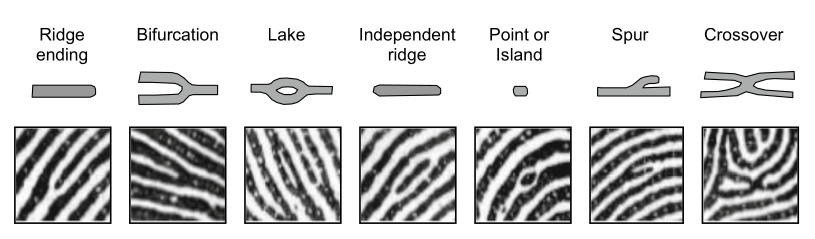
\includegraphics[width=0.65\textwidth]
	{minutiae_types}
	\caption{Seven most common minutiae types}
\end{figure}

\newpage The points in which these discontinuities or changes in ridge pattern occur, are referred to as minutiae points. Minutiae points possess several inherent attributes, but we will only need a few of them for our purposes. Each minutiae point has the following primary attributes include: X-Y cartesian coordinates, minutiae orientation, minutiae type, and a confidence score.

\begin{figure}[H]
	\centering
	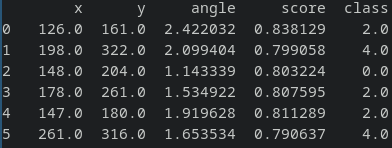
\includegraphics[width=0.4\textwidth]
	{minutiae_pandas}
	\caption{A list of detected minutiae points and their attributes}
\end{figure}

The cartesian coordinates are the pixel coordinates of the minutiae point's location on the fingerprint input image. The orientation of a minutiae, is the direction it is heading towards, or in other words the direction of the line tangent to the ridge at that point. The minutiae type is an integer enumeration of the seven most common types of minutiae as referred to in Figure 2.1. The confidence score, is the probability of that minutiae point being a legitimate minutiae point, according to the FingerFlow framework, which we will discuss in the next chapter.

\subsection{Delaunay Triangulation}
Considering a set of discrete points $P$ on a euclidean plane, a three-point subset:

\begin{center}
	$\{p_1, p_2, p_3\} \subset P$
\end{center}
 is considered a Delaunay Triangle, if and only if no other point in $P$ is inside the circumcircle of the three-point subset. \cite{delaunay34trig}
 
\begin{figure}[H]
	\centering
	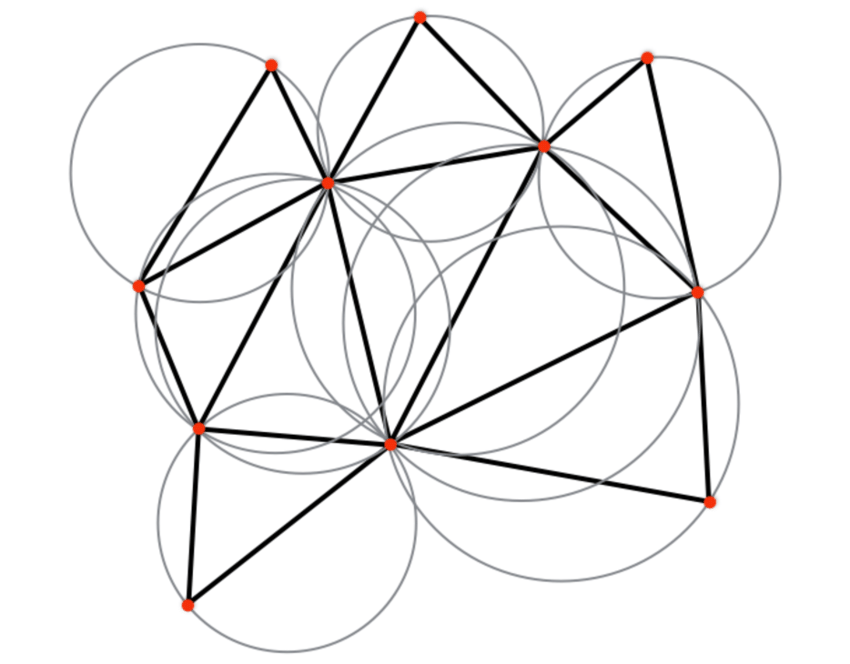
\includegraphics[width=0.35\textwidth]
	{delaunay}
	\caption{A set of points subjected to Delaunay Triangulation}
\end{figure}

After deriving all feasible Delaunay Triangles from the points in $P$, we end up with a connected graph of neighboring triangles with no intersecting edges. There are many algorithms with which to perform Delaunay Triangulation with:

\subsubsection{Voronoi Algorithm}
Given a set of $n$ discrete points $P = \{p_1, p_2, ..., p_n\}$ on a Euclidean plane, the plane is segmented into $n$ non-overlapping partitions dedicated to each point in $P$. Each of these partitions is referred to as a Voronoi cell.  Every Voronoi cell $C_k$, consists of every point on the plane for which its respective point $p_k$ is the closest site. Meaning the distance of any arbitrary point within $C_k$ is minimal from itself to $p_k$ than to any other point $p_i \ne p_k$. The set of all Voronoi cells, make up a Voronoi diagram.

\begin{figure}[H]
	\centering
	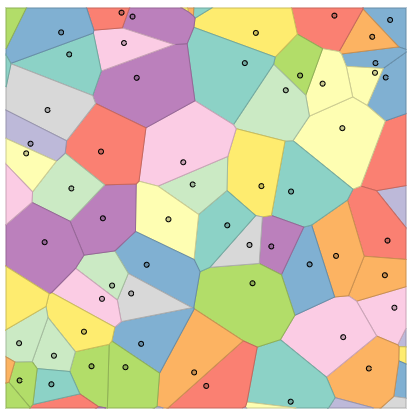
\includegraphics[width=0.4\textwidth]
	{voronoi}
	\caption{A Voronoi diagram consisting of Voronoi cells and their respective points}
\end{figure}

The borders of these Voronoi cells, refered to as Voronoi edges, are constructed by creating the perpendicular bisector of the line between two points respectively and blending them. Finally, the Delaunay Triangulation of $P$ is then created by connecting the points of all neighboring Voronoi cells. The Yang method originally uses the Voronoi algorithm to derive the Delaunay Triangles from the set of minutiae points on a fingerprint. But there is another easier to implement algorithm which was used in our implementation instead.

\subsubsection{The Bowyer-Watson Algorithm}
In computational geometry, the Bowyer-Watson algorithm is an incremental algorithm for deriving all possible Delaunay Triangles from a set of points in N-dimensional Euclidean space. The pseudo-code is fully described in \ref{code:a1}. The complexity for this algorithm is $O(n log(n))$ if implemented efficiently, and $O(n^2)$ in a normal sub-optimal implementation. The Python implementation of the Bowyer-Watson algorithm was readily available from a Python package named \texttt{delaunay-triangulation} \cite{delgit}, which was imported and used in our code.

\begin{figure}[H]
	\centering
	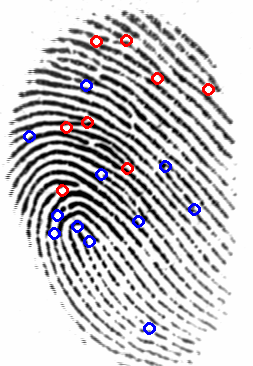
\includegraphics[width=0.2\textwidth]
	{minutiae_points}
	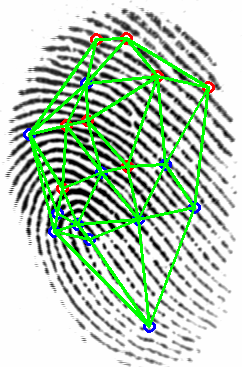
\includegraphics[width=0.191\textwidth]
	{minutiae_del}
	\caption{Minutiae points on a fingerprint and its Delaunay Triangulation}
\end{figure}

\section{The Yang Method}
\subsection{Brief Outline}
The Yang method's outline follows from general outline described in \ref{sol}, and includes the mentioned Enrolment and Verification phases. The generation of the IFT from the fingerprint image, is done separately in parallel under two different schemes: The Polar Coordinate-based scheme and the Delaunay Triangulation-based scheme.

The Polar IFT, which is an array of vectors with zero and one entries, is then transformed using the Feature Decorrelation Algorithm (FDA) (which will be discussed in Chapter 3), and then projected into a lower dimension using a projection matrix pseudo-randomly generated from a seed. The seed used to generate the pseudo-random projection matrix, is a part of the Public Key associated with the TFT. Every vector in the Polar IFT, is essentially based around a reference minutiae point and its polar coordinate-based relations with other minutiae points within a certain predefined radius. Therefore within the Polar IFT, there's a vector dedicated to every minutiae point, since every vector is created by setting a minutiae point as the origin point.

The Delaunay IFT, is essentially an array of all Delaunay Triangles encoded and quantized into binary numbers, based on attributes such as side length, the angle between two sides of the triangle, the minutiae type of the triangle vertices, and orientation differences between two vertices. Thereafter, the Delaunay IFT is permutated into the Delaunay TFT by converting each encoded triangle in the IFT from binary to integer, and adding it to another integer which is generated based on a predetermined integer $\phi$. The $\phi$ number is another part of the Public Key associated with the TFT.

After the two IFTs of the target fingerprint are obtained, we obtain the two IFTs of the query fingerprint using the same Public Key (same projection matrix and $\phi$). Then the similarity scores of the respective IFTs are calculated (\texttt{SC\_MAX} for the Polar IFTs, and \texttt{SD} for the Delaunay IFTs), normalized, and put into a Final Score formula for giving the finalized similarity score of the two fingerprints.

\subsection{Advantages}
The main contributions of the Yang method compared to the previously mentioned works, involve the following advantages:

\subsubsection{Reduced Non-Linear Distortion}
Since the Yang method's IFT and final result depend on a combination of the Polar Coordinate-based and Delaunay Triangulation-based schemes, the impact of non-linear distortion, which would lead to recognition inaccuracy being reduced. Roughly speaking, non-linear distortion results from systems in which the output signal is not exactly proportional to the input signal. 

For instance a cause of non-linear distortion would be to have a system which solely relies on the Polar Coordinate-based scheme for the generation of its IFT, which would result in the system not taking into account the minutiae that are located far away from the reference minutiae. That is because, in the Polar Coordinate-based scheme, only minutiae that are placed within a certain limited radius of the reference minutiae are taken into account and used to generate the IFT. Therefore, compared with the system that solely uses a Polar Coordinate-based scheme, higher recognition accuracy is achieved.

\subsubsection{ARM Attack Invulnerability}
The ARM attack, otherwise known as attack via record multiplicity, is an exploit which results from the compromise of several TFTs and their respective generative parameters (the Public Key in our case), and leads to the full or partial generation of the original IFT. A main reason that a lot of Cancelable Biometrics methods suffer from the ARM attack is due to feature correlation. To propagate this issue, a FDA is implemented within the method, so that in the process of the IFT to TFT transformation, the feature vectors within the IFT become uncorrelated in regards to another. Without any correlation between said features in the IFT, the attacker wouldn't have enough data to determine the original IFT.

\subsection{Guarantee of Irreversibility}
\subsection{Guarantee of Comparability}

\chapter{Algorithm and Implementation}
\section{The Algorithm in Full Detail}
\section{Used Tools}
\section{Implementation}

\chapter{Evaluation}
\section{Recognition Accuracy of FingerFlow}
\section{Recognition Accuracy of the Yang Method}
\section{Performance Analysis}

\chapter{Conclusion}

\section{Future Work}

\bibliographystyle{socreport}
\bibliography{socreport}

\appendix
\chapter{Code}
\section{Bowyer-Watson Pseudo-Code}
\label{code:a1}
\begin{lstlisting}
	def BowyerWatson (pointList):
		#pointList is a set of coordinates defining the points to be triangulated
		triangulation := empty triangle mesh data structure
		# must be large enough to completely contain all the points in pointList
		add super-triangle to triangulation 
		# add all the points one at a time to the triangulation
		for each point in pointList: 
			badTriangles := empty set
			# first find all the triangles that are no longer valid due to the insertion
			for each triangle in triangulation: 
				if point is inside circumcircle of triangle:
					add triangle to badTriangles
			polygon := empty set
			# find the boundary of the polygonal hole
			for each triangle in badTriangles: 
				for each edge in triangle:
					if edge is not shared by any other triangles in badTriangles:
						add edge to polygon
			# remove them from the data structure
			for each triangle in badTriangles:
				remove triangle from triangulation
			# re-triangulate the polygonal hole
			for each edge in polygon:
				newTri := form a triangle from edge to point
				add newTri to triangulation
		# done inserting points, now clean up
		for each triangle in triangulation:
			if triangle contains a vertex from original super-triangle:
				remove triangle from triangulation
		return triangulation
\end{lstlisting}

\end{document}
